\chapter{\xlabel{manual}Running \task{makemap} Outside the Pipeline}
\label{sec:manual}

The previous chapter described how to make maps using the SCUBA-2 Pipeline.
Users - particularly new users - are encourage to use the pipeline for
their map-making. However, greater control of the map-making
process is available by running the \makemap\ command directly, rather
than from within the pipeline. This chapter describes how to do this, but
should be seen as ``advanced usage''.

\begin{quote}
\emph{
Note, when \makemap\ is run manually (rather than from the pipeline) the
resulting image will be in units of pW, not Jy. Each pixel value
in the map represents the weighted mean value of the bolometer samples
(in pW) that fall within the pixel, after removal of the noise components
described in \cref{Section}{sec:models}{The individual models}. Each
weight is the reciprocal of the variance associated with the bolometer.
Thus each pixel value can be thought of as the astronomical power
received by a typical bolometer at each point on the sky.
\cref{Section}{sec:cmult}{Flux conversion factors} describes how to
convert a map from units of pW to Jy.
}
\end{quote}

\section{Running \texttt{makemap}}

Before running \makemap\ directly, you need to ensure that the Starlink
environment has been initialised and the \smurf\ package started (see
\cref{Section}{sec:starinit}{Initialising Starlink} and
\cref{Section}{sec:packinit}{KAPPA and SMURF for data processing}).

To run \makemap, you  need to supply values for the following
command-line parameters\footnote{Note the distinction between
``command-line parameters'' (also known as ``ADAM'' parameters) that are
supplied on the \texttt{makemap} command line, and ``configuration parameters''
that are specified within a configuration file. Values for all
\emph{configuration} parameters are obtained using a single \emph{command-line}
parameter called \texttt{CONFIG}.}:

\begin{itemize}

\item \texttt{IN} - a list of input NDFs containing raw SCUBA-2 data (see
\cref{Section}{sec:rawdata}{The raw data} and \cref{Section}{sec:ndf}
{Data formats}). There are many ways in which the list of files can be supplied,
as described in Section ``\xref{Specifying Groups of Objects}{sun95}{se_groups}''
in \xref{SUN/95}{sun95}{}. The easiest is to create a simple text
file containing the names of the raw data files -- one per line --- and
then supply the name of the text file, preceded by an up-caret character
(\,\texttt{\^{}}\,), as the value for parameter \texttt{IN}. Note, the names of
the raw data files can contain wild-cards such as ``$*$'' and ``?''.

\item \texttt{OUT} - the name of the NDF in which to store the final
map. The supplied file name should either have a file type of
``\texttt{.sdf}'', or no file type at all (in which case \texttt{.sdf}
will be appended to the supplied value). Any existing file with the same
name will be over-written.

\item \texttt{CONFIG} - a string that specifies new values for one or more
configuration parameters. These new values are used in place of the
\xref{default values}{sun258}{par_full} described in
\xref{SUN/258}{sun258}{}. Any configuration parameter not specified by
the \texttt{CONFIG} string retains its default value. As with files
names, there are many ways in which the group of parameter values can be
specified, and the same documentation should be consulted for details
(\xref{SUN/95}{sun95}{se_groups}). Again, the easiest way is to list the
parameter values in a simple text file with one parameter setting (a
``<name>=<value>'' string) on each line. See \cref{Section}{sec:config}
{Specialised configuration files} for a list of the pre-defined
configuration files that come with \smurf. Note, \texttt{CONFIG}
can be set to the special value ``\texttt{def}'' to force \makemap\ to
use the default values for all parameters. It \emph{is} possible to create
a map using just these default values, but it will not usually be a very
good map. Advice on which parameters to edit can be found in
\cref{Section}{sec:tweak}{Tweaking the configuration file}.

\end{itemize}

If any of the above parameters are \emph{not} given on the \texttt{makemap}
command line, prompts will be issued and the user invited to supply values
for the missing parameters.

So an example command line would be:
\begin{terminalv}
% makemap in=^myfiles.lis out=850_crl2688 \
          config=^$STARLINK_DIR/share/smurf/dimmconfig_bright_compact.lis
\end{terminalv}

Here, the file \texttt{myfiles.lis} contains a list of the raw data
files to be included in the map, and could for instance look like this:

\begin{terminalv}
% cat myfiles.lis
/jcmtdata/raw/scuba2/s8a/20120720/00030/*
/jcmtdata/raw/scuba2/s8b/20120720/00030/*
/jcmtdata/raw/scuba2/s8c/20120720/00030/*
/jcmtdata/raw/scuba2/s8d/20120720/00030/*
\end{terminalv}

This uses all available data for all four 850\,$\mu$m sub-arrays, for
observation 30 taken on 20th July 2012\footnote{The input files should all be
for a single waveband and a single observation --- do not mix files from
different wavebands and/or observations.}.

The file \brightcompact\ is one of the pre-defined configuration files
supplied with \smurf. It contains configuration parameter values that are
optimised for creating maps from bright compact sources.

\begin{tip}
  An up-caret (\,\texttt{\^{}}\,) is required any time you are reading
  in a group text file in \starlink. For the map-maker this includes
  the configuration file (a group of configuration parameters) and the
  list of input files ( a group of NDFs --- \emph{e.g.}  \texttt{in=\^{}\,myfiles.lis}).
\end{tip}

After the \texttt{makemap} command completes, the final map will be left in file
\texttt{850\_crl2688.sdf} and can be displayed using \gaia:

\begin{terminalv}
% gaia 850_crl2688
\end{terminalv}

There are many other command-line parameters that can be supplied when
running \texttt{makemap}, but only the three listed above are mandatory. All the
others assume default values if not supplied on the command-line. For a
full list of all available command-line parameters, their functions and
default values, see the description of \makemap\ within the \textsc{smurf}
document, \xref{SUN/258}{sun258}{}.

You can supply values for any of these extra parameter on the command
line. For instance, one of the command-line parameters that is usually
defaulted is \texttt{PIXSIZE}, which specifies the pixel size for the final
map, in arc-seconds. The default pixel sizes, defined as one quarter of the
Airy disk rounded up to the nearest half arc-second, are:

\begin{itemize}
\item 2\,arcsec at 450$\mu$m
\item 4\,arcsec at 850$\mu$m
\end{itemize}

So for instance, the above command-line could be modified as follows to
produce a map with 3 arc-second pixels:

\begin{terminalv}
% makemap in=^myfiles.lis out=850_crl2688 pixsize=3 \
          config=^$STARLINK_DIR/share/smurf_bright_compact.lis
\end{terminalv}

Note, if parameters are specified by name on the command-line, as
in these examples, then the order in which they are specified is
insignificant\footnote{Some commands, for instance most \textsc{Kappa}
commands, allow the most important parameters to be specified by position
rather than name, in which case their order \emph{is} significant ---
see \xref{\texttt{Specifying Parameter Values on Command Lines}}{sun95}
{se_cmdlindef} in \xref{SUN/95}{sun95}{}.}. Also, parameter names are
case-insensitive.

\begin{tip}
  Map-maker not finding your raw data files from a path? Check you have
  escaped or protected any shell meta-characters in your `in' value,
  for instance by putting double quotes around it or escaping
  wild-cards using a backslash (\emph{e.g.} ``\texttt{in=\textbackslash*.sdf}''
  or just ``\texttt{in=\textbackslash*}''). Note, this issue applies only to
  wild-cards included directly on the command line --- there is no need to
  escape or protect wild cards within a text file.
\end{tip}

\section{Interpreting the screen output from \task{makemap}}

Whilst \makemap\ runs, it outputs information continuously to the screen
about what it is doing. The amount of information displayed can be
controlled using the \xref{\texttt{MSG\_FILTER}}{sun258}{sec_msg} command-line
parameter. It defaults to ``\texttt{normal}'', but if you want more
information you could set it to (say) ``\texttt{verbose}'':

\begin{terminalv}
% makemap in=^myfiles.lis out=850_crl2688 msg_filter=verb \
          config=^$STARLINK_DIR/share/smurf_bright_compact.lis
\end{terminalv}

Note - unambiguous abbreviations may be used for many command line
parameters --- so ``\texttt{verb}'' is acceptable instead of
``\texttt{verbose}''. Setting \texttt{MSG\_FILTER} to ``\texttt{quiet}''
will suppress all screen output.

\begin{tip}
  Map-maker generates a lot of screen output! The main things to check
  are that the ``\texttt{NORMALIZED MAP CHANGE}'' value (the mean value,
  not the max value) decreases nicely towards your requested
  \xparam{MAPTOL}{maptol} value as each iteration is completed, and that
  the ``\texttt{Total samples available for map:}'' value does not fall
  too low (you should usually be looking for values above 50\% of
  maximum). If neither of these two items look problematic, it is usually
  safe to pay less attention to the other screen output.
\end{tip}

The following shows the screen output generated by a typical run of \makemap\
if \texttt{MSG\_FILTER} is left set to its default value of
``\texttt{normal}''. Explanatory comments, which are not actually
part of the output generated by \makemap, are included in \emph{emphasised
type}. The input data is a short observation of a bright compact source
(CRL 2688):

\begin{terminalv}
% makemap in=^myfiles.lis out=850_crl2688 \
          config=^$STARLINK_DIR/share/smurf_bright_compact.lis

Out of 32 input files, 4 were darks, 8 were fast flats and 20 were science
Processing data from instrument 'SCUBA-2' for object 'CRL2688' from the
following observation  :
  20120720 #30 scan
\end{terminalv}

\emph{The output starts by reporting information about the input data files,
including the number that contain on-sky bolometer values (``science''
data), the astronomical object and the SCUBA-2 observation number.}

~
\begin{terminalv}

MAKEMAP: Map-maker will use no more than 92586 MiB of memory

   Projection parameters used:
      CRPIX1 = 0
      CRPIX2 = 0
      CRVAL1 = 315.578333333333 ( RA = 21:02:18.800 )
      CRVAL2 = 36.6938055555556 ( Dec = 36:41:37.70 )
      CDELT1 = -0.00111111111111111 ( -4 arcsec )
      CDELT2 = 0.00111111111111111 ( 4 arcsec )
      CROTA2 = 0

   Output map pixel bounds: ( -132:122, -126:129 )

   Output map WCS bounds:
        Right ascension: 21:01:38.318 -> 21:03:03.280
        Declination: 36:33:07.19 -> 36:50:11.70
\end{terminalv}

\emph{Next comes information about the output map. The world coordinate
system is described by means of the equivalent \htmladdnormallink{FITS-WCS}
{http://fits.gsfc.nasa.gov/fits_wcs.html} keywords\footnote{In fact, NDF
data structures do not use FITS-WCS to describe WCS --- instead they use the
\htmladdnormallink{AST}{http://www.starlink.ac.uk/ast} library, which
provides a much more flexible scheme for handling WCS.}}

\emph{The reported pixel bounds of the output map refer to a pixel coordinate
system in which the source is centred at position (0,0). Note, the definition of
pixel coordinates within the NDF format allows the origin of pixel
coordinates to be at any nominated position within the array --- it does
not have to be at the bottom left corner as in FITS --- and \texttt{makemap}
chooses to put the pixel origin at the specified source position. }

\emph{Finally, the bounds of the map are given in the celestial coordinate
system specified by the \xref{\texttt{SYSTEM}}{sun258}{MAKEMAP} command-line
parameter.  This parameter defaults to ``\texttt{tracking}'', which causes
the map to be created in the celestial coordinate system in which the
observation parameters were originally defined. It may instead be set to a
specific coordinate system (e.g. ``galactic'', ``icrs'', etc.) to force the
map to be made in that system.}

~
\begin{terminalv}
smf_iteratemap: will down-sample data to match angular scale of 4 arcsec
smf_iteratemap: Iterate to convergence (max 40)
smf_iteratemap: stop when mean normalized map change < 0.05
\end{terminalv}

\emph{By default, the data is down-sampled so that the on-sky distance between
adjacent samples is roughly equal to the pixel size (4 arc-seconds in
this case). This saves memory and computing time without adversely
affecting the final map. The degree of down-sampling can be controlled
using the \xparam{DOWNSAMPSCALE}{downsampscale} configuration parameter.}

\emph{Next come information about the stopping criteria for the iterative
map-making algorithm. In this case, iterations will stop when 40 iterations are
completed, or the normalised change in the map between iterations reduces
to less that 0.05. These values are specified by configuration parameters
\xparam{NUMITER}{numiter} and \xparam{MAPTOL}{maptol} (see \cref{Section}
{sec:converge}{Stopping criteria}).}

~
\begin{terminalv}
smf_iteratemap: provided data are in 1 continuous chunks, the largest of which
has 5957 samples (153.729 s)
smf_iteratemap: map-making requires 1626 MiB (map=28 MiB model calc=1598 MiB)
smf_iteratemap: Continuous chunk 1 / 1 =========
\end{terminalv}

\emph{In almost all cases, the raw data files constituting a SCUBA-2
observation will correspond to a single continuous stream of data
samples, taken at roughly 200 Hz. Sometimes however, this may not be the
case\footnote{A common cause of this is if some sub-scans are omitted
from the list of input files supplied to \task{makemap}.}, so the user is
now told how many chunks of data were found, and how long they were.
Something may be wrong if the input data contains any breaks.}

\emph{Next comes information about the amount of memory needed to make
the map. If insufficient memory is available to process all the input
data together, it will be split into chunks, and a separate map made from
each chunk. These maps are later co-added to form the final output map.
This can often result in a poorer map --- see \latexhtml{the box
describing \emph{Data Chunking} on Page~\pageref{box:chunk})~}
{\htmlref{Data Chunking)}{box:chunk}}.}

\emph{Finally, a loop is entered to process each chunk in turn, and the
user is told which chunk is currently being processed. In this
case there  is only one chunk (which is good).}

~
\begin{terminalv}
smf_iteratemap: Iteration 1 / 40 ---------------
\end{terminalv}

We now start the first iteration of the iterative algorithm described in
\cref{Section}{sec:algorithm}{The reduction step-by-step}, to create a
map from the current chunk of  input data. We will be performing ----
at most --- 40 iterations, as set by \xparam{NUMITER}{numiter}.

~
\begin{terminalv}
--- Size of the entire data array ------------------------------------------
bolos  : 5120
tslices: 5957(2.6 min)
Total samples: 30499840
\begin{terminalv}
--- Quality flagging statistics --------------------------------------------
 BADDA:   10805998 (35.43%),        1814 bolos
BADBOL:   10865568 (35.62%),        1824 bolos
DCJUMP:      19631 ( 0.06%),
  STAT:      71680 ( 0.24%),          14 tslices
 NOISE:      41699 ( 0.14%),           7 bolos
Total samples available for map:   19586411, 64.22% of max (3287.97 bolos)
\end{terminalv}

\emph{Now we have a number of statistics describing the cleaned data
prior to the first iteration\footnote{Setting
\texttt{MSG\_FILTER=verbose} on the \texttt{makemap} command line will
generate more information about the cleaning process.}.}

\emph{Each sub-array contains a grid of $32\times40$ bolometers, making 5120
bolometers in total over all four sub-arrays. The number of time slices in
the concatenated data after down-sampling is reported. In this case, 5957
time slices over 2.6 minutes, equating to a down-sampled frequency of about
38 Hz. The total number of samples is the product of the number of
bolometers and the number of time slices. Each of the following lines
indicates the percentage of the data that has been flagged as unusable for
various reasons:}

\begin{itemize}
\item \emph{BADDA - flagged as unusable during data acquisition.}
\item \emph{DCJUMP - flagged as unusable because of a sudden step change in
the base-line.}
\item \emph{STAT - flagged as unusable because the telescope was stationary
(or at least moving too slowly).}
\item \emph{NOISE - flagged as unusable because they were too noisy.}
\end{itemize}

\emph{The BADBOL item gives the fraction of bolometers that have been
flagged as entirely bad for any of these reasons, and from which no data
will be used.}

~
\begin{terminalv}
smf_iteratemap: Calculate time-stream model components
smf_iteratemap: Rebin residual to estimate MAP
smf_iteratemap: Calculate ast
\end{terminalv}

\emph{Indicates the models that are being calculated. More information
about each individual model is displayed if you set
\texttt{MSG\_FILTER=verbose} on the \texttt{makemap} command line.}

~
\begin{terminalv}
--- Quality flagging statistics --------------------------------------------
 BADDA:   10805998 (35.43%),        1814 bolos  ,change          0 (+0.00%)
BADBOL:   11008536 (36.09%),        1848 bolos  ,change     142968 (+1.32%)
DCJUMP:      19631 ( 0.06%),                    ,change          0 (+0.00%)
  STAT:      71680 ( 0.24%),          14 tslices,change          0 (+0.00%)
   COM:     372786 ( 1.22%),                    ,change     372786 (+0.00%)
 NOISE:      41699 ( 0.14%),           7 bolos  ,change          0 (+0.00%)
Total samples available for map:   19214687, 63.00% of max (3225.56 bolos)
     Change from last report:    -371724, -1.90% of previous
smf_iteratemap: Will calculate chi^2 next iteration
smf_iteratemap: *** NORMALIZED MAP CHANGE: 2.22778 (mean) 60.5292 (max)
\end{terminalv}

\emph{More statistics are displayed once the first iteration is completed
and the first estimate of the science map has been generated. Data
samples may be flagged as bad within the iterative stage for various
reasons, and so these statistics may be different to those shown prior to
the start of the iterative stage. Most significantly, the \texttt{COM:}
line shows the percentage of data that has been rejected because the time
stream did not resemble the common-mode signal closely enough. The
``\texttt{NORMALIZED MAP CHANGE}'' values are of no real significance on the
first iteration since there is no previous map with which to compare the
new map (in fact the numerical values are generated by comparing the new map
with a map full of zeros).}

~
\begin{terminalv}
smf_iteratemap: Iteration 2 / 40 ---------------
smf_iteratemap: Calculate time-stream model components
smf_calcmodel_noi: Calculating a NOI variance for each box of 581 samples
using variance of neighbouring residuals.
smf_iteratemap: Rebin residual to estimate MAP
smf_iteratemap: Calculate ast
--- Quality flagging statistics --------------------------------------------
 BADDA:   10805998 (35.43%),        1814 bolos  ,change          0 (+0.00%)
BADBOL:   11038321 (36.19%),        1853 bolos  ,change      29785 (+0.27%)
 SPIKE:         36 ( 0.00%),                    ,change         36 (+0.00%)
DCJUMP:      19631 ( 0.06%),                    ,change          0 (+0.00%)
  STAT:      71680 ( 0.24%),          14 tslices,change          0 (+0.00%)
   COM:     393125 ( 1.29%),                    ,change      20339 (+5.46%)
 NOISE:      41699 ( 0.14%),           7 bolos  ,change          0 (+0.00%)
Total samples available for map:   19194401, 62.93% of max (3222.16 bolos)
     Change from last report:     -20286, -0.11% of previous
smf_iteratemap: *** CHISQUARED = 0.997314089857974
smf_iteratemap: *** NORMALIZED MAP CHANGE: 1.78691 (mean) 8.09056 (max)

\end{terminalv}

\emph{The second iteration starts, and proceeds in much the same way as the
first iteration. The main difference is that the NOI model is generated
at the start of the second iteration. This model measures the variance
within each bolometer time-stream. It is used to weight the bolometer
samples when forming the mean sample value in each map
pixel\footnote{Bolometers are given equal weight in the map created at
the end of the first iteration since the NOI model has not yet been
calculated at that point.}. NOI is calculated from the residuals left after
removal of all other models, and is only calculated once --- subsequent
iterations re-use the same NOI values.}

\emph{The \texttt{SPIKE:} item that has appeared in the quality flagging
statistics records the number of samples that have been rejected as
transient spikes in the time-series. This flagging is done by comparing
the bolometer values that fall in each map pixel, and flagging any that
appear to be statistical out-liers - see configuration parameter
\xparam{AST.MAPSPIKE}{ast.mapspike}.}

\emph{The mean ``\texttt{NORMALIZED MAP CHANGE}'' value should drop with each
subsequent iteration (note, the ``max'' normalised map change value
can usually be ignored as it records the maximum normalised change in any
single map pixel and is thus highly subject to random variations).}

~
\begin{terminalv}
smf_iteratemap: Iteration 3 / 40 ---------------
smf_iteratemap: Calculate time-stream model components
smf_iteratemap: Rebin residual to estimate MAP
smf_iteratemap: Calculate ast
--- Quality flagging statistics --------------------------------------------
 BADDA:   10805998 (35.43%),        1814 bolos  ,change          0 (+0.00%)
BADBOL:   11050235 (36.23%),        1855 bolos  ,change      11914 (+0.11%)
 SPIKE:         36 ( 0.00%),                    ,change          0 (+0.00%)
DCJUMP:      19631 ( 0.06%),                    ,change          0 (+0.00%)
  STAT:      71680 ( 0.24%),          14 tslices,change          0 (+0.00%)
   COM:     401600 ( 1.32%),                    ,change       8475 (+2.16%)
 NOISE:      41699 ( 0.14%),           7 bolos  ,change          0 (+0.00%)
Total samples available for map:   19185947, 62.91% of max (3220.74 bolos)
     Change from last report:      -8454, -0.04% of previous
smf_iteratemap: *** CHISQUARED = 0.976599086972009
smf_iteratemap: *** change: -0.0207150028859653
smf_iteratemap: *** NORMALIZED MAP CHANGE: 0.305 (mean) 1.24407 (max)
\end{terminalv}

\emph{The mean normalised map change continues to drop with the third
iteration, as expected. The total number of samples going into the map is
dropping with each iteration, but only very slowly. This is mainly due to
the increased number of samples being flagged by the COM model, but is at
an acceptably small level.}

~
\begin{terminalv}
smf_iteratemap: Iteration 4 / 40 ---------------
smf_iteratemap: Calculate time-stream model components
smf_iteratemap: Rebin residual to estimate MAP
smf_iteratemap: Calculate ast
--- Quality flagging statistics --------------------------------------------
 BADDA:   10805998 (35.43%),        1814 bolos  ,change          0 (+0.00%)
BADBOL:   11056192 (36.25%),        1856 bolos  ,change       5957 (+0.05%)
 SPIKE:         36 ( 0.00%),                    ,change          0 (+0.00%)
DCJUMP:      19631 ( 0.06%),                    ,change          0 (+0.00%)
  STAT:      71680 ( 0.24%),          14 tslices,change          0 (+0.00%)
   COM:     409883 ( 1.34%),                    ,change       8283 (+2.06%)
 NOISE:      41699 ( 0.14%),           7 bolos  ,change          0 (+0.00%)
Total samples available for map:   19177684, 62.88% of max (3219.35 bolos)
     Change from last report:      -8263, -0.04% of previous
smf_iteratemap: *** CHISQUARED = 0.96404406922676
smf_iteratemap: *** change: -0.0125550177452489
smf_iteratemap: *** NORMALIZED MAP CHANGE: 0.0401588 (mean) 0.151877 (max)
\end{terminalv}

\emph{After the fourth iteration the mean normalised map change has
dropped to 0.0401588, which is below the value of 0.05 provided for the
\xparam{MAPTOL}{maptol} parameter by the \brightcompact\
configuration file\footnote{In fact, 0.05 is the default \texttt{maptol}
value, which is left unchanged by \texttt{dimmconfig\_bright\_compact.lis}.}.
Consequently, \texttt{makemap} considers the map to have converged. However,
in view of the fact that the \brightcompact\ configuration file uses
``AST masking'' (see \cref{Section}{sec:astmask}{AST masking}), it is
necessary to do one final iteration in order to assign correct values to
the pixels that lie outside the source mask. Note, when AST masking is being
used, the reported normalised map change values only include pixels that
are within the source mask.}

~
\begin{terminalv}
smf_iteratemap: Iteration 5 / 40 ---------------
smf_iteratemap: Calculate time-stream model components
smf_iteratemap: Rebin residual to estimate MAP
smf_iteratemap: Calculate ast
--- Quality flagging statistics --------------------------------------------
 BADDA:   10805998 (35.43%),        1814 bolos  ,change          0 (+0.00%)
BADBOL:   11068106 (36.29%),        1858 bolos  ,change      11914 (+0.11%)
 SPIKE:         36 ( 0.00%),                    ,change          0 (+0.00%)
DCJUMP:      19631 ( 0.06%),                    ,change          0 (+0.00%)
  STAT:      71680 ( 0.24%),          14 tslices,change          0 (+0.00%)
   COM:     414727 ( 1.36%),                    ,change       4844 (+1.18%)
 NOISE:      41699 ( 0.14%),           7 bolos  ,change          0 (+0.00%)
Total samples available for map:   19172853, 62.86% of max (3218.54 bolos)
     Change from last report:      -4831, -0.03% of previous
smf_iteratemap: *** CHISQUARED = 0.964032127175568
smf_iteratemap: *** change: -1.19420511923707e-05
smf_iteratemap: *** NORMALIZED MAP CHANGE: 0.0157131 (mean) 0.103135 (max)
smf_iteratemap: ****** Completed in 5 iterations
smf_iteratemap: ****** Solution CONVERGED
Setting 24282 map pixels bad because they contain fewer than 4 samples (=0.01
of the mean samples per pixel).
Total samples available from all chunks: 19172853 (3218.54 bolos)
\end{terminalv}

\emph{After the extra iteration required by AST masking has been
performed, the final output map is created. It is always advisable to
check the final number of samples available for the map, as a low value
will cause your map to have high noise levels. In this case, 62.86\% of
the samples are available for the map, which is quite acceptable --- only
a couple of percent of the samples have been rejected by the map-making,
mostly flagged by the COM model. The bulk of the bad samples (35.43\%)
were rejected during data acquisition due to dead bolometers \emph{etc}.}

\emph{Note, the \xparam{NUMITER}{numiter} parameter is set to -40 by
\brightcompact, meaning that no more than 40 iterations will be
performed. In this particular case we only needed 4 iteration (plus a
mandatory extra iteration) to achieve
our requested \xparam{MAPTOL}{maptol} value. But it is possible for some
observations --- particularly observations of extended sources --- to
require more than 40 iterations to converge to a \texttt{maptol} of 0.05.
In such cases the screen output will end with a message saying that the
solution ``FAILED TO CONVERGE''\footnote{However a map will still be
created, but should be used with caution.}. In such cases, you \emph{could}
simply increase \texttt{numiter} and re-run \texttt{makemap}, but you may
also want to investigate the cause of the slow convergence using one or more
of the techniques described in \cref{Chapter}{sec:raw}{Chapter 9}, as it
may indicate some issue with the raw data.}

\emph{Map pixels that receive a very small number of samples are automatically
set bad. These are usually the pixels around the periphery of the
observation, and will have very unreliable variance estimates. The
threshold is determined by the \xparam{HITSLIMIT}{hitslimit} parameter,
which defaults to 1 percent of the mean number of hits per pixel,
corresponding to 4 samples per pixel in this case.}

\emph{The observation used in this particular case was a short
observation of a calibrator, lasting only 2.6 minutes. Consequently there
was no need to divide the data up into multiple chunks in order to fit it
into memory.  However, for very long observations, or for shorter
observations when using a computer with less than the recommended amount
of memory (see \cref{Section}{sec:computing}{Chapter 1}), it may be
necessary to process the raw data in multiple chunks. If this happens, a
map is created from each chunk in turn, and all these maps are then added
together to form the final map.  The final message ``\texttt{Total
samples available from all chunks: 19172853 (3218.54 bolos)}'' indicates
the total number of samples (and equivalent number of bolometers) used
from all chunks. In this case there was only one chunk, so these values
are equal to the numbers reported at the end of the last iteration.}

\section{Interacting with \texttt{makemap} during a long run}
For long observations, \makemap\ can take several hour to run,
particularly on slow or low memory computers. For this reason it is
useful to be able to monitor progress so that potential problems can be
detected early, in order to avoid wasting time.

\subsection{Monitoring screen output}
The most straight-forward way of monitoring progress is to check the
values written to the screen by \texttt{makemap} at the end of each iteration (see
the previous section). For instance, if you run \texttt{makemap} as follows:

\begin{terminalv}
% makemap in=^infiles out=outmap config=^conf | tee makemap.log
\end{terminalv}

then the messages displayed by makemap on the screen will also be written
to text file \texttt{makemap.log}. This makes it easy to search the log
file whilst \texttt{makemap} is still running, for instance from another terminal
window:

\begin{terminalv}
% grep NORMALIZED makemap.log
smf_iteratemap: *** NORMALIZED MAP CHANGE: 1.02829 (mean) 20.7922 (max)
smf_iteratemap: *** NORMALIZED MAP CHANGE: 0.739832 (mean) 9.81836 (max)
smf_iteratemap: *** NORMALIZED MAP CHANGE: 0.370128 (mean) 5.42933 (max)
smf_iteratemap: *** NORMALIZED MAP CHANGE: 0.258304 (mean) 3.2717 (max)
smf_iteratemap: *** NORMALIZED MAP CHANGE: 0.205415 (mean) 2.66815 (max)
smf_iteratemap: *** NORMALIZED MAP CHANGE: 0.177044 (mean) 2.28417 (max)
smf_iteratemap: *** NORMALIZED MAP CHANGE: 0.159569 (mean) 2.05803 (max)
\end{terminalv}

This displays the normalised change in maps between successive
iterations, for the iterations that have so far been completed. If the mean
normalised map change is not decreasing smoothly,
(for instance if it is oscillating around a fixed value), then there is a
potential problem. In which case you may want to interrupt the
\texttt{makemap} process, rather than waiting potentially for several
hours just to end up with a bad map.

Likewise, it is useful to monitor the total number of samples that are
being pasted into the map at the end of each iteration:

\begin{terminalv}
% grep "Total samples" makemap.log
Total samples: 299919360
Total samples available for map:  174105275, 58.05% of max (2972.2 bolos)
Total samples available for map:  171284110, 57.11% of max (2924.03 bolos)
Total samples available for map:  171242020, 57.10% of max (2923.32 bolos)
Total samples available for map:  171239147, 57.10% of max (2923.27 bolos)
\end{terminalv}

The lower the percentage of samples included in the map, the greater will
be the noise in the map. If this number drops much below 50\% then you
may want to think about aborting \texttt{makemap} and investigating why
the number is so low (\emph{e.g.} by looking at the ``quality
statistics'' displayed at the end of each iteration, to determine the
cause of the data loss).

Likewise, information can be gather about chunking:

\begin{terminalv}
% grep chunk makemap.log
smf_iteratemap: provided data are in 7 continuous chunks, the largest of
which has 487 samples (10.1534 s)
smf_iteratemap: Continuous chunk 1 / 7 =========
smf_iteratemap: Adding map estimated from this continuous chunk to total
smf_iteratemap: Continuous chunk 2 / 7 =========
smf_iteratemap: Adding map estimated from this continuous chunk to total
smf_iteratemap: Continuous chunk 3 / 7 =========
smf_iteratemap: Adding map estimated from this continuous chunk to total
\end{terminalv}

This indicates that the raw data has gaps in it, resulting in seven maps
being made, one from each continuous chunk, before the final map is made
by combining all the individual maps. Chunking can produce sub-optimal
maps, and should normally be investigated - see \latexhtml{the description
of \emph{Data Chunking} on Page~\pageref{box:chunk})~}{\htmlref{Data
Chunking}{box:chunk}}.

\subsection{Monitoring the map at the end of each iteration}
\label{sec:itermaps}
The map created at the end of each iteration is normally discarded, but can
be saved by setting configuration parameter \xparam{ITERMAP}{itermap}
to either 1 or 2. By default, these ``itermaps'' are written to an
extension of the main output NDF as described in
\cref{Section}{sec:inter}{Writing out models and intermediate maps}, and
cannot be viewed until \makemap\ has completed. However, an alternative
destination for these itermaps can be specified on the \texttt{makemap}
command-line as follows, allowing them to be viewed whilst \texttt{makemap}
is still running:

\begin{terminalv}
% cat conf
^STARLINK_DIR/share/smurf/dimmconfig_jsa_generic.lis
itermap=1
%
% makemap in=^infiles out=outmap config=^conf itermaps=myitermaps
\end{terminalv}

Note the distinction between the ``\texttt{itermaps}'' (plural)
\emph{command-line} option, and the ``\texttt{itermap}'' (singular)
\emph{configuration} parameter.  As soon as the first iteration has
finished, the above command will create a new file
called \texttt{myitermaps.sdf} in which each itermap will be stored as soon
as it is created. The file is closed after each itermap is written, and
re-opened again before writing the next itermap. This is an example of a
\emph{container file}, where a single \texttt{.sdf} file contains several
NDFs, each holding a different map (see \cref{Section}{sec:ndf}{Data
formats}). You can list the maps in such a file using \textsc{Kappa}
\xref{\task{ndfecho}}{sun95}{NDFECHO} as follows:

\begin{terminalv}
% ndfecho myitermaps
myitermaps.CH00I001
myitermaps.CH00I002
myitermaps.CH00I003
myitermaps.CH00I004
myitermaps.CH00I005
myitermaps.CH00I006
myitermaps.CH00I007
...
\end{terminalv}

The name of each itermap is of the form ``CHxxIyyy'', where ``xx'' is the
chunk number and ``yyy'' is the iteration number. In the common case
where all raw data is processed in a single chunk, ``xx'' will be ``00''
for all itermaps.

You can view a single itermap using:
\begin{terminalv}
% gaia myitermaps.CH00I004
\end{terminalv}

If you want to view several itermaps side-by-side, you can use \textsc{Kappa}
\xref{\task{picgrid}}{sun95}{PICGRID} to divide the screen up into a grid
of ``pictures'', then use \xref{\task{picsel}}{sun95}{PICSEL} to pick each
picture in turn, and use \xref{\task{display}}{sun95}{DISPLAY} to display
an itermap in each one. For instance to display the first six itermaps
side-by-side in a $3 \times 2$ grid, all with the same scaling, without
any axes, do:

\begin{terminalv}
% gdclear
% picgrid 3 2
% picsel 1
% display myitermaps.CH00I001 axes=no mode=percentiles percentiles=\[2,98\]
% picsel 2
% display myitermaps.CH00I002 mode=current
% picsel 3
% display myitermaps.CH00I003 mode=current
% picsel 4
% display myitermaps.CH00I004 mode=current
% picsel 5
% display myitermaps.CH00I005 mode=current
% picsel 6
% display myitermaps.CH00I006 mode=current
\end{terminalv}

This produces the display shown in \cref{Figure}{fig:itermaps}{Initial
six itermaps}. \textsc{Kappa} \xref{\task{display}}{sun95}{DISPLAY} has
many options for controlling things like data scaling, axis annotation
and style, colour table, graphics device, \emph{etc.}.

\begin{figure}
\begin{center}
  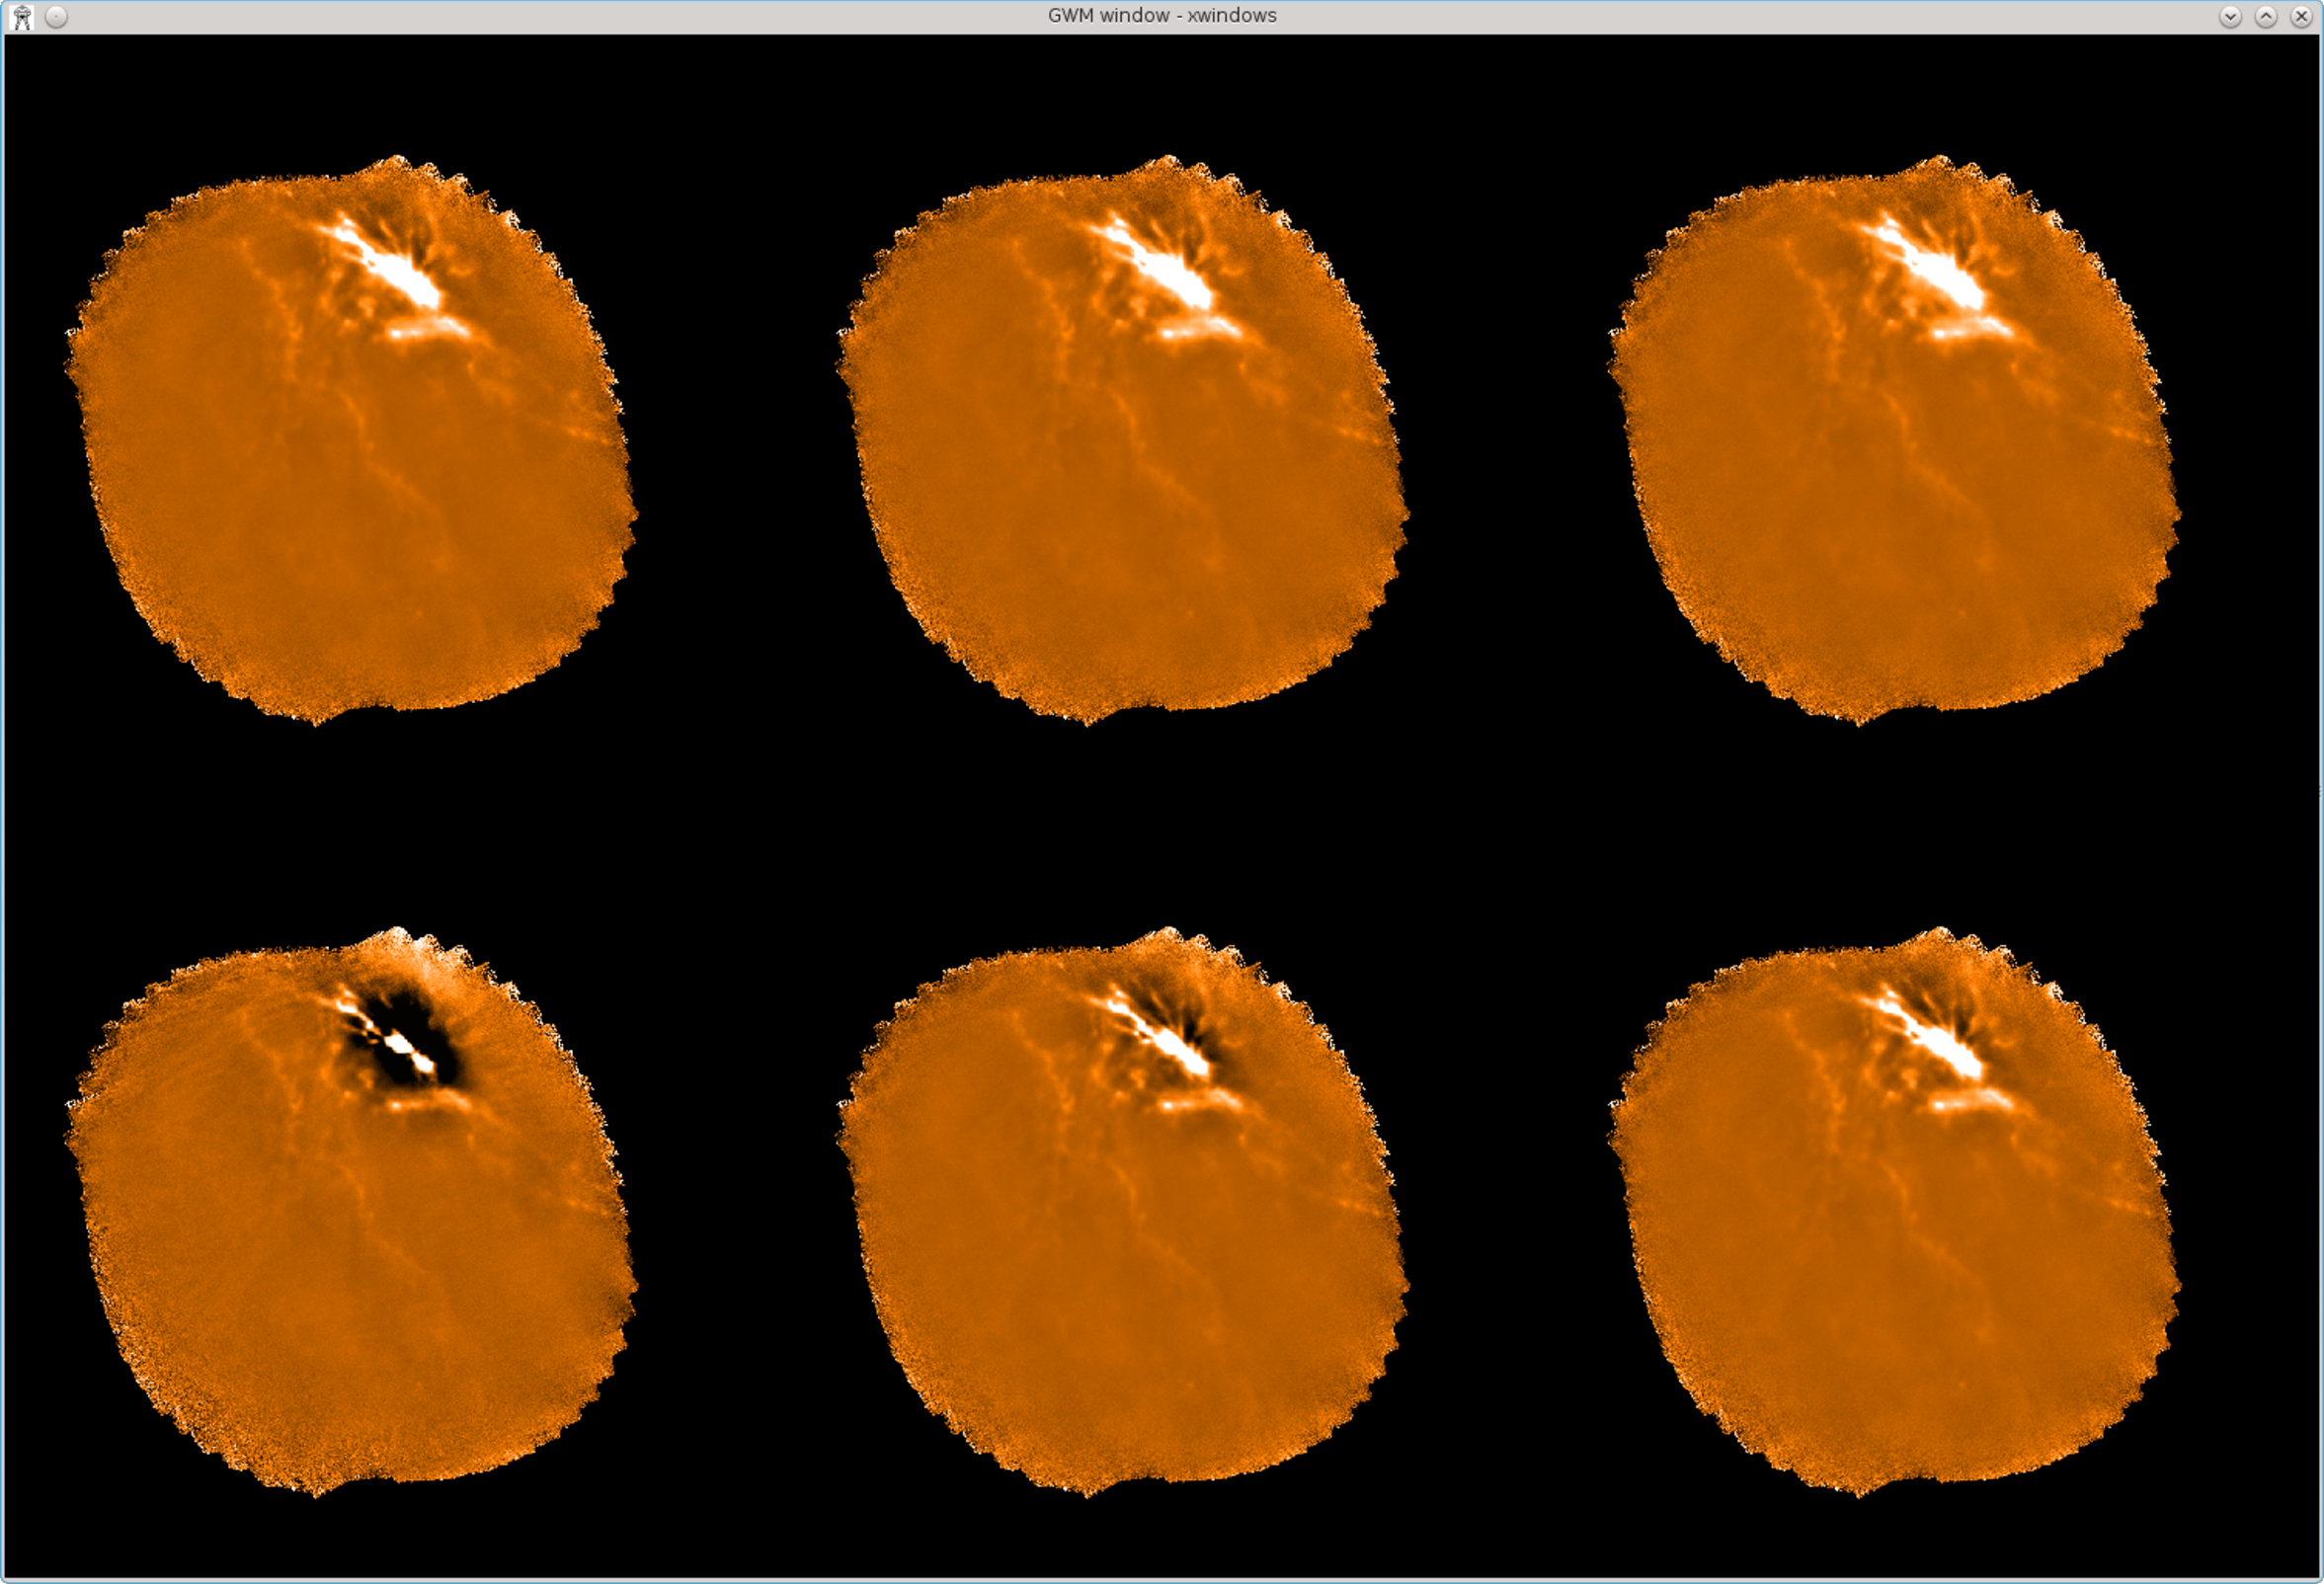
\includegraphics[width=\linewidth]{sc21_itermaps}
\end{center}
\caption[Initial six itermaps]{\small The maps created on the first six
iterations of \texttt{makemap}, from an observation of Orion A, using the
\texttt{dimmconfig\_jsa\_generic.lis} configuration file with the addition
of ``\texttt{itermap=1}''. The first map is bottom left, and the sixth
map is top right. This illustrates the initial fast improvement
in the map over the first few iterations.}
\label{fig:itermaps}
\end{figure}

Alternatively, you can combine the itermaps into a 3D cube, and then use
the cube-viewing facilities of \gaia\ to scroll through the itermaps in the
style of a movie (see \cref{Section}{sec:inter}{Writing out models and
intermediate maps})\footnote{Note, \textsc{smurf} \stackframes\ can be used
instead of \textsc{Kappa} \xref{\task{paste}}{sun95}{PASTE} if preferred.}:

\begin{terminalv}
% paste in=myitermaps out=itercube shift=\[0,0,1\]
% gaia itercube
\end{terminalv}

It is sometimes informative
to look at the \emph{change} between
itermaps, to see the incremental effect of each iteration. This is most
easily done if the itermaps are first stacked into a cube as described
above. The next step is to produce a copy of the cube in which the pixel
origin is moved by one pixel along the third axis (\emph{i.e.} the axis
that enumerates iteration). Finally subtract one cube from the other, and
display the resulting difference cube (this example shows how command-line
parameters can often be specified by position instead of by name when
running \textsc{Kappa} commands --- check the help information for each
command to see the order in which options should be supplied):

\begin{terminalv}
% paste myitermaps out=itercube shift=\[0,0,1\]
% slide itercube itercube-shifted \[0,0,1\] near
% sub itercube-shifted itercube diffcube
%
% picsel 1
% display diffcube'(,,1)' axes=no mode=percentiles percentiles=\[2,98\]
% picsel 2
% display diffcube'(,,2)' mode=current
% picsel 3
% display diffcube'(,,3)' mode=current
% picsel 4
% display diffcube'(,,4)' mode=current
% picsel 5
% display diffcube'(,,5)' mode=current
% picsel 6
% display diffcube'(,,6)' mode=current
\end{terminalv}

This produces the display shown in \cref{Figure}{fig:diffmaps}{Initial
six difference maps}.

\begin{figure}
\begin{center}
  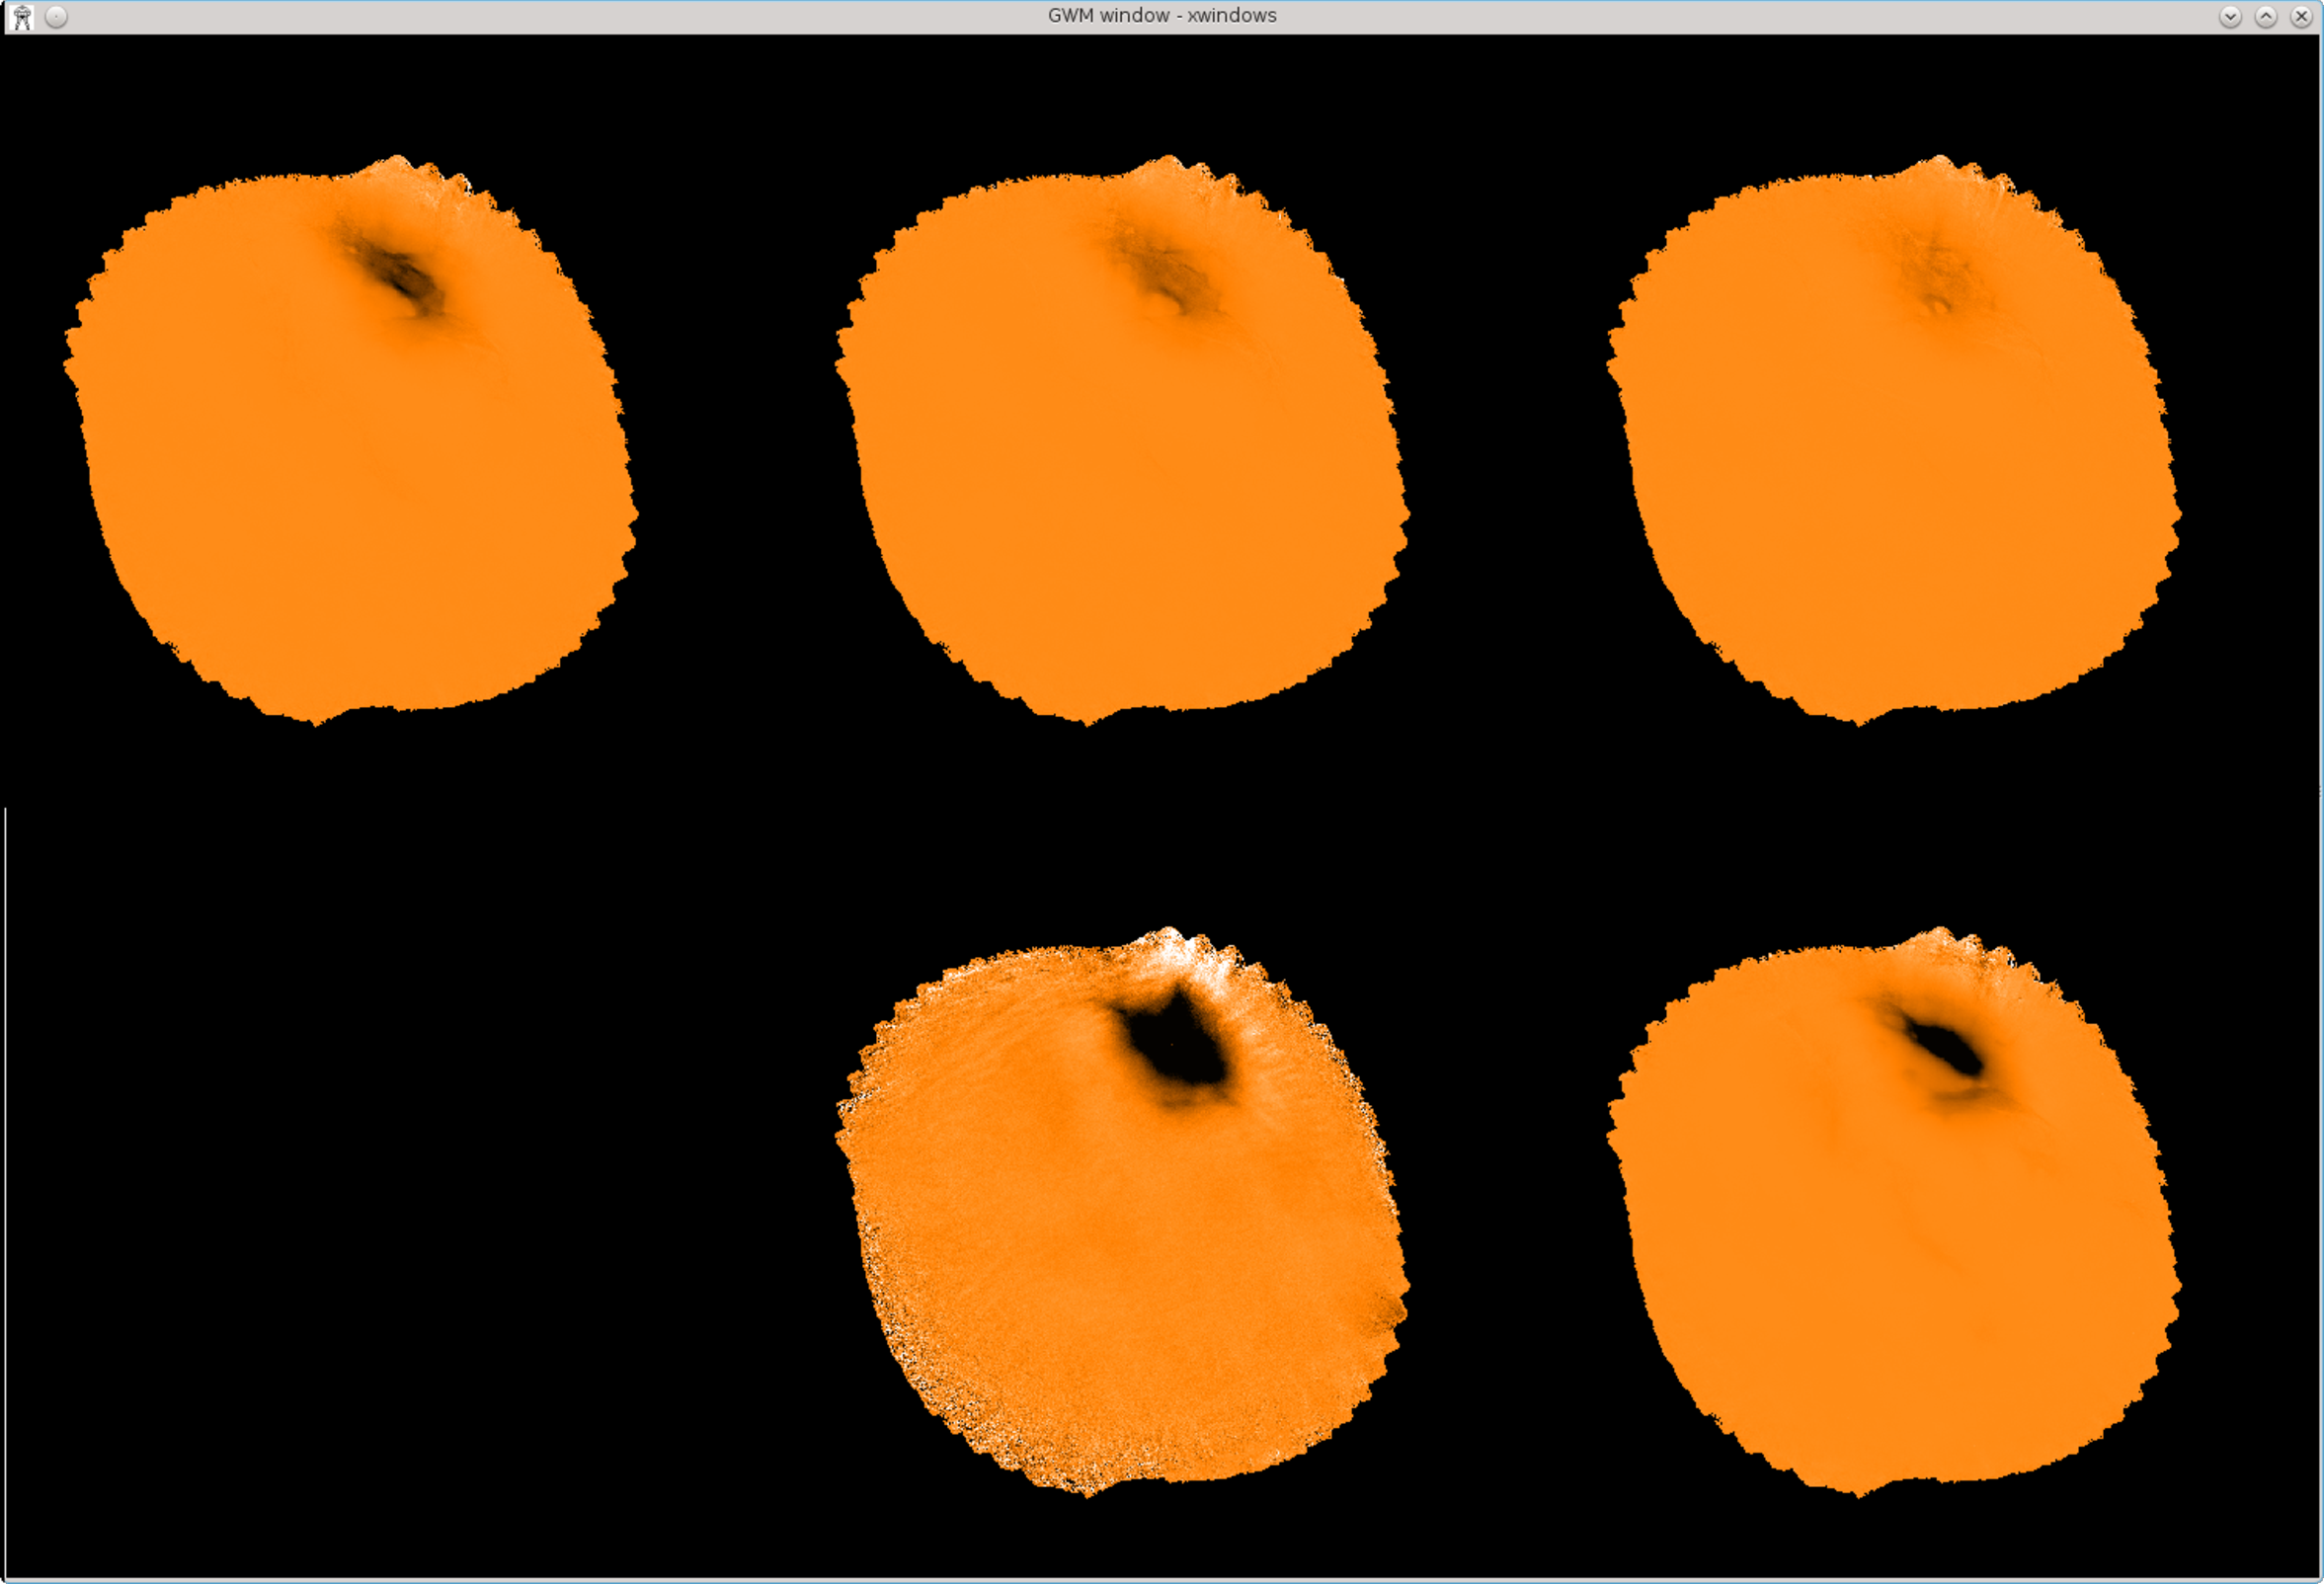
\includegraphics[width=\linewidth]{sc21_diffmaps}
\end{center}
\caption[Initial six difference maps]{\small The difference between each
pair of adjacent maps shown in \cref{Figure}{fig:itermaps}{Initial
six itermaps}.}
\label{fig:diffmaps}
\end{figure}

\textbf{Viewing the mask after each iteration:}

The above plots are based on the itermaps that are created by adding
``\texttt{itermaps=1}'' to your \texttt{makemap} configuration. You can
instead use ``\texttt{itermaps=2}'', which causes each itermap to be
masked so that pixels outside the current source mask are set bad
(\emph{i.e.} blank)\footnote{If no masking is being used, then
\texttt{itermaps=2} has the same effect as \texttt{itermaps=1}.}.
\cref{Figure}{fig:maskeditermaps}{Initial six itermaps with masking}
shows the resulting itermaps.

\begin{figure}
\begin{center}
  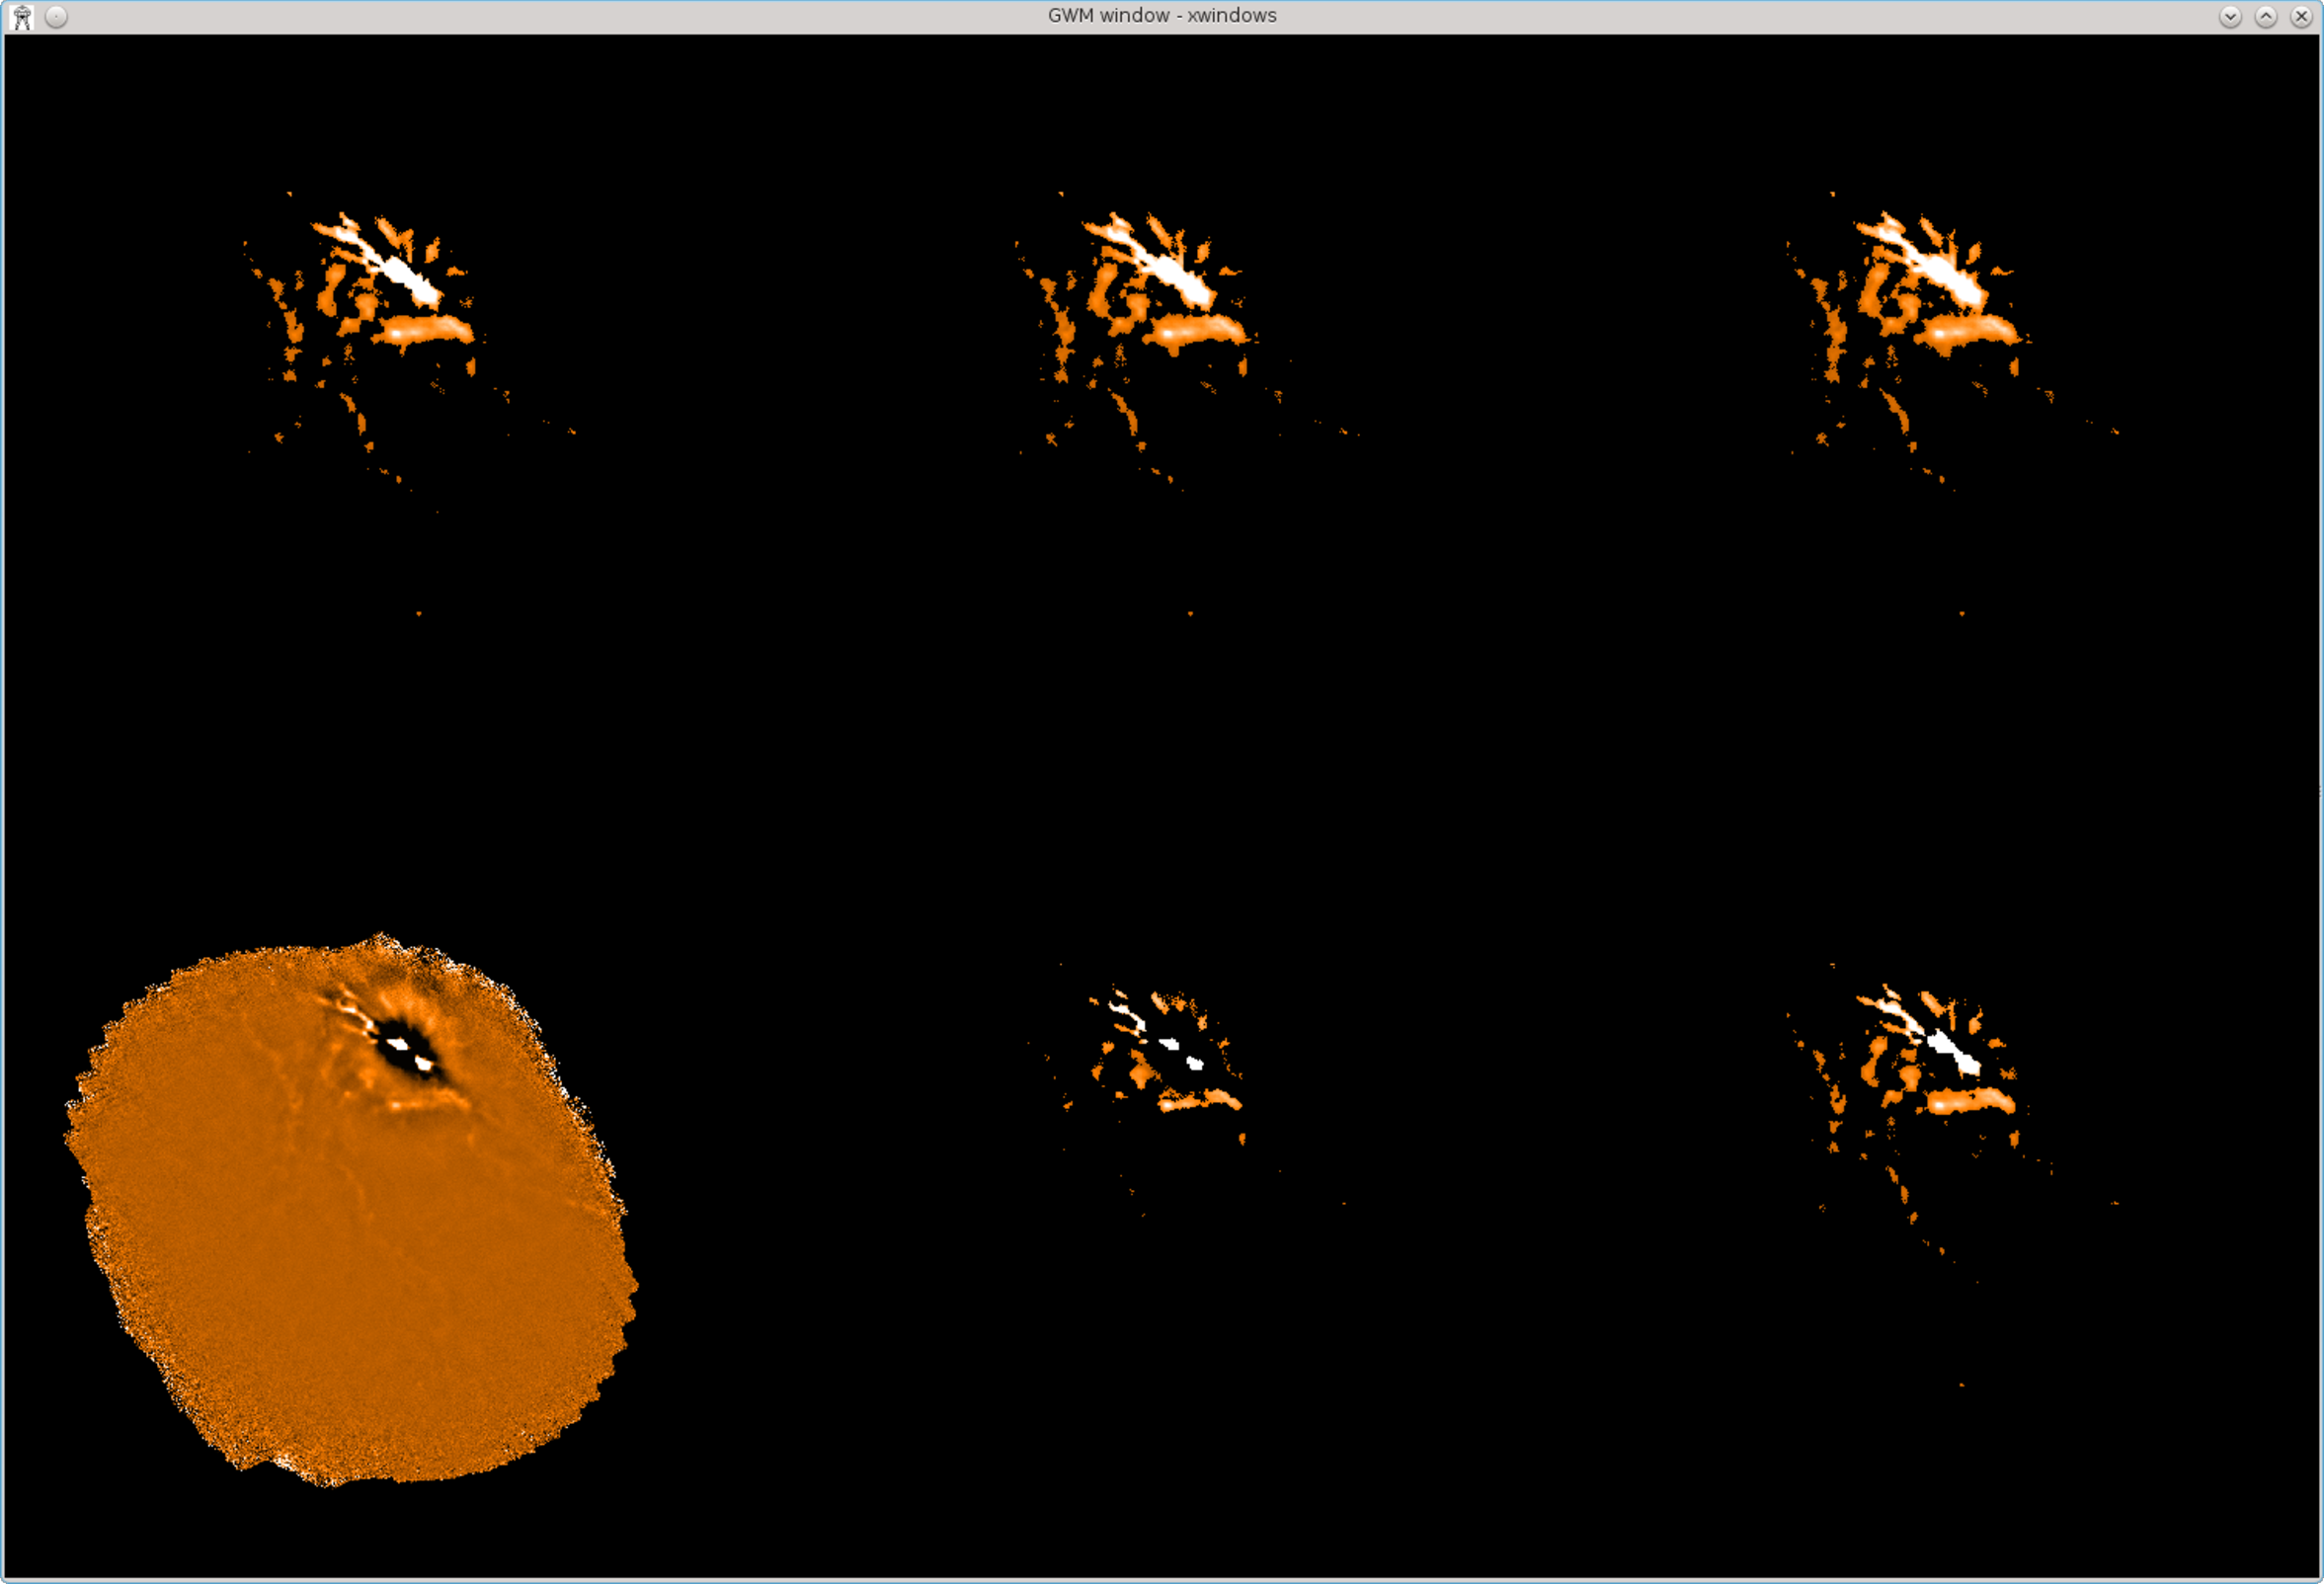
\includegraphics[width=\linewidth]{sc21_itermaps_masked}
\end{center}
\caption[Initial six itermaps with masking]{\small The first six
itermaps, create by using \texttt{itermap=2} in the configuration. This
causes pixels outside the source mask to be set blank, allowing the evolution
off the mask to be seen (the first iteration is not masked). In this
case, the mask includes all pixels above a signal-to-noise ratio of five.}
\label{fig:maskeditermaps}
\end{figure}

The main point of this section is to emphasise that all the above
investigations can be performed \emph{whilst makemap is still running},
if you specify an explicit file for the itermaps using the
``\texttt{itermaps} command-line option. This allows you to decide if
the reduction is progressing as expected, and whether to interrupt the
reduction.


\subsection{Interrupting \texttt{makemap}}

If you interrupt \makemap\ by pressing control-C on the keyboard (or
equivalently by sending an \texttt{INT} signal to the \texttt{makemap}
process), it will continue until the current iteration is completed
and then will issue a prompt with options allowing you to save the current
map before closing, as in the following example:

\begin{terminalv}
% makemap in=^infiles out=outmap config=^conf itermaps=myitermaps
Out of 29 input files, 1 was a dark, 1 was a fast flat and 27 were science
Processing data from instrument 'SCUBA-2' for object 'OMC1 tile10' from the
following observation  :
...
...
\end{terminalv}

\texttt{<press control-C>}

\begin{terminalv}
...
...
--- Quality flagging statistics
--------------------------------------------
 BADDA:   25525734 (20.86%),         267 bolos  ,change          0 (+0.00%)
BADBOL:   31261854 (25.55%),         327 bolos  ,change          0 (+0.00%)
 SPIKE:        339 ( 0.00%),                    ,change          4 (+1.19%)
DCJUMP:     146703 ( 0.12%),                    ,change          0 (+0.00%)
  STAT:     160000 ( 0.13%),         125 tslices,change          0 (+0.00%)
   COM:    1827454 ( 1.49%),                    ,change       3000 (+0.16%)
 NOISE:    5640518 ( 4.61%),          59 bolos  ,change          0 (+0.00%)
Total samples available for map:   89135553, 72.84% of max (932.361 bolos)
     Change from last report:      -3001, -0.00% of previous
smf_iteratemap: *** CHISQUARED = 0.998314983615372
smf_iteratemap: *** change: -0.0014711436109287
smf_iteratemap: *** NORMALIZED MAP CHANGE: 0.00941492 (mean) 2.9521 (max)


>>>> Interrupt detected!!! What should we do now? Options are:
1 - abort immediately with an error status
2 - close the application returning the current output map
3 - do one more iteration to finalise the map and then close

NOTE - another interrupt will abort the application, potentially leaving
files in an unclean state.

INTOPTION - What to do now (1-3) /3/ >
\end{terminalv}

At this point you should respond to the prompt for parameter
\texttt{INTOPTION} by typing 1, 2 or 3 followed by \texttt{<return>}. Options 2
and 3 cause \texttt{makemap} to tidy up its internals and create a map
from the current models just as if the iterative process had reached
convergence. Option 3 causes one further iteration to be performed,
without masking (you should use this option if you have been using AST
masking --- see \cref{Section}{sec:astmask}{AST masking}).

\begin{tip}
Note if you are running \texttt{makemap} from within a script, then the
handling of control-C interrupts will probably be quite different, because
the shell process (or perl, python or whatever) will catch the interrupt
before it gets to the \texttt{makemap} process. This usually causes the
shell process to die but leaves the \texttt{makemap} process running in
the background. Instead of pressing control-C on the keyboard, you should
find the process ID for the \texttt{makemap} process itself, and then send an
INT signal to that process explicitly:

\begin{terminalv}

% ps aux | grep makemap
dsb      25407  0.0  0.0  43716  1952 pts/5    0:00 makemap
% kill -s INT 25407

\end{terminalv}

\end{tip}


\section{Tips and Tricks}
\subsection{Aligning your map with a pre-existing image}
If you want to compare SCUBA-2 data with a map of the same region taken
with a different instrument, you will usually want to create the
SCUBA-2 map using the same pixel grid as the other map so that you can
compare pixel values directly in the two maps\footnote{Creating the map on the
required pixel grid is better than creating it on a default grid and then
re-sampling it onto the required grid later.}. You can use the
\aparam{REF} command-line parameter to do this. For instance, if your
other map is in file \texttt{herschel.sdf}, you can do:

\begin{terminalv}
% makemap in=^infiles out=outmap config=^conf ref=herschel
\end{terminalv}

This will cause the output map in file \texttt{outmap.sdf} to use
the same pixel grid as \texttt{herschel.sdf}.  This means that a given
point on the sky will have the same \emph{pixel coordinates} in both
maps, and so for instance you could divide one by the other to get a
ratio map without any further alignment step:

\begin{terminalv}
% div outmap herschel ratio_map
\end{terminalv}

This will divide \texttt{outmap.sdf} by \texttt{herschel.sdf} and put the
ratio in \texttt{ratio\_map.sdf}\footnote{In reality you would probably
want to take account of differing resolutions and /or units in the two
maps before dividing them.}.

However, by default \texttt{makemap} will trim the output map to
exclude blank borders, thus the two maps may have different
\emph{dimensions}. NDF-based applications such as \textsc{Kappa}
\xref{\task{div}}{sun95}{DIV} automatically take account of this when
comparing corresponding pixels in two NDFs --- see
\cref{Figure}{fig:pixelco}{Pixel coordinates}.

\begin{figure}
\begin{center}
  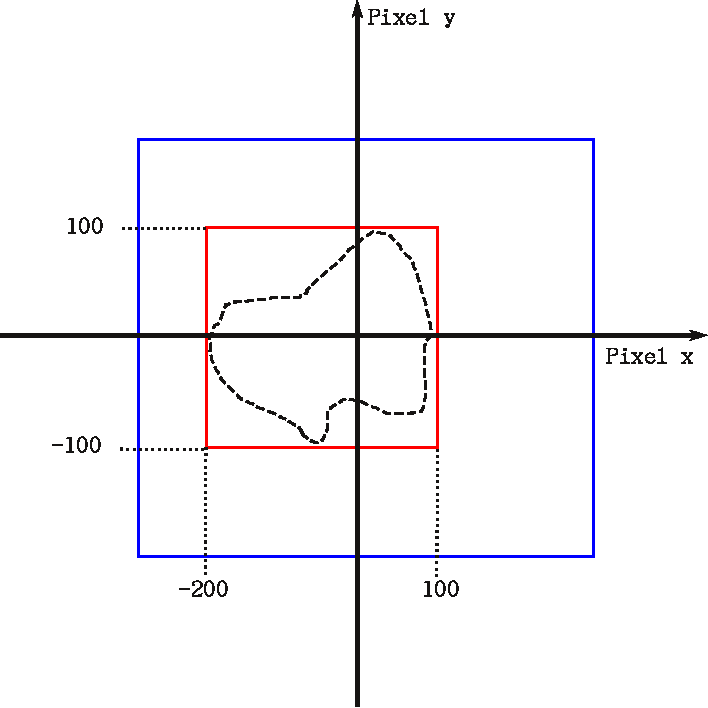
\includegraphics[width=0.8\linewidth]{sc21_pixelco}
\end{center}
\caption[Pixel coordinates]{\small The curved dotted line represents a
contour of an astronomical object. The heavy black lines represent the
X and Y axes of the pixel coordinate system, crossing at the pixel origin
(\texttt{pixel\_x},\texttt{pixel\_y})=(0,0). The numerical values
represent pixel X and Y values. The blue box represents the
bounds of the reference map supplied when running makemap. The
red box represents the bounds of the map created by makemap.
The reference image and the output image share the same pixel
coordinate system, so a given point on the sky has the same pixel
coordinates in both images. However, the output (red) image is cropped to
remove blank borders and so has smaller dimensions than the reference
(blue) image. All this is made possible by the fact that the NDF format, unlike
FITS, does not require the origin of pixel coordinates to be at the
bottom left corner of each map. NDF applications account for any
difference in pixel origin when comparing pixels in different files.}
 \label{fig:pixelco}
\end{figure}

If you want to force the output map to have certain bounds in pixel
coordinates, you can do so by assigning values to the \aparam{LBND} and
\aparam{UBND} parameters when running \texttt{makemap}. For instance, if
you want to force the output map to have the same dimensions as the
reference map, you could use \textsc{Kappa} \xref{\task{ndftrace}}{sun95}{NDFTRACE}
to list the properties of the reference NDF, including its pixel bounds, and
then assign these bounds to \aparam{LBND} and \aparam{UBND} parameters when
running \texttt{makemap}:

\begin{terminalv}
% ndftrace herschel

   NDF structure /home/dberry/herschel1:
      Title:  Example Herschel data

   Shape:
      No. of dimensions:  2
      Dimension size(s):  351 x 400
      Pixel bounds     :  -50:300, 1:400
      Total pixels     :  140400
...
...
% makemap in=^infiles out=outmap config=^conf ref=herschel \
          lbnd=\[-50,1\] ubnd=\[300,400\]
\end{terminalv}

The resulting map in \texttt{outmap.sdf} will have the same pixel bounds
as \texttt{hershel.sdf}.

\subsection{Limiting the amount of memory used by \texttt{makemap}}
There may be occasions when you need to limit the amount of memory used
by \makemap\ --- for instance to leave enough memory for other processes
to function correctly. For machines with more than 20 GB of memory, the
default is to leave 4 GB free for other processes. For machines with less
than than 20 GB of memory, the default is to leave 20\% of the total
memory free. This default can be over-ridden by indicating the maximum
amount of memory that \texttt{makemap} should use by setting a value for
the command-line parameter \aparam{MAXMEM}. For instance:

\begin{terminalv}
% makemap in=^infiles out=outmap config=^conf maxmem=50000
\end{terminalv}

will ensure that \texttt{makemap} never uses more than 50000
MiB\footnote{One MiB is 1048576 bytes.} of memory. Be aware though that
for larger observations this may cause the data to be processed in
multiple chunks rather than a single continuous chunk, resulting in a
poorer map.

\subsection{Re-using previously cleaned data to speed up map-making}
\label{sec:reuse}

Usually, you will create your SCUBA-2 maps using one of the standard
configuration files distributed with \textsc{smurf} (see
\cref{Section}{sec:config} {Specialised configuration files}). However,
for certain problematic observations it may sometimes be necessary to
experiment with several different configurations to find one that
produces an acceptable map. In such cases a significant amount of time
can be saved by re-using pre-cleaned raw data each time you make a map,
rather than re-cleaning it each time.

By default \makemap\ assumes that the supplied data is raw data that
requires cleaning before being used to make a map. However, if you include
``\setparam{DOCLEAN}{doclean}{0}'' in your configuration, then
\texttt{makemap} will skip the entire cleaning process and move directly
on to the iterative map-making stage, thus saving significant time.

Obviously though, in this case you need to make sure that the data you
supply to \texttt{makemap} has already been cleaned. There are two ways
to do get cleaned data:

\begin{enumerate}

\item You can run \texttt{makemap} initially on the \emph{un}-cleaned
data (\emph{i.e.} the original raw data), and force \texttt{makemap} to
dump the cleaned data to disk before going onto the iterative map-making
stage. You can then re-use this cleaned data in subsequent invocations of
\texttt{makemap}. To dump the cleaned data, you need to add
``\setparam{EXPORTCLEAN}{exportclean}{1}'' to the configuration on your
initial run of \texttt{makemap} --- don't forget to remove it for
subsequent runs! The cleaned data are put into files in the current
directory, one for each sub-array, with names such as
\texttt{s8c20120706\_00037\_0003\_con\_res\_cln.sdf}. Note the \texttt{\_cln} on
the end of the name indicating cleaned data. The base name,
``\texttt{s8c20120706\_00037\_0003}'' in this case, is taken from the first
raw data file that contributes to each chunk. If the entire observation
is processed in one chunk (as it should usually be) then there will be
one such \texttt{\_cln} file for each sub-array. If the observation is
split into multiple chunks, then there will be multiple  \texttt{\_cln} files
for each sub-array (one for each chunk).

\item You can use the separate \smurf\ task \clean\ to clean the data
as described in \cref{Appendix}{app:clean}{Cleaning the raw data}.

\end{enumerate}





